\section[Solution 1: Probability Refresher I]{Solution 1: Probability Refresher I \iftoggle{showdates}{\small{\textit{2014-04-28}}}{}}

\subsection*{Exercise 2}
\index{Odds}

\subsubsection*{Exercise 2.a}

We use the formula for calculating odds:
\begin{align*}
\frac{p}{1-p} = \frac{s_2}{s_1}
\end{align*}
The probability for rolling a 6 is $\frac{1}{6}$, $s_1$ can be set to 10.
\begin{align*}
\frac{\frac{1}{6}}{1-\frac{1}{6}} = \frac{s_2}{10} \Leftrightarrow s_2 = 2
\end{align*}
So our stake should be \$2.


\subsubsection*{Exercise 2.b}
We use the same formula again, this time with $s_1=25$.
\begin{align*}
\frac{\frac{1}{6}}{1-\frac{1}{6}} = \frac{s_2}{25} \Leftrightarrow s_2 = 5
\end{align*}
So we accept all stakes $s_2 \geq \$ 5$.


\subsubsection*{Exercise 2.c}
We use the formula for odds and solve it for $p$.
\begin{align*}
                & & \frac{p}{1 - p} & = \frac{s_2}{s_1}                     & & \\
\Leftrightarrow & & p               & = \frac{s_2}{s_1} (1 - p)             & & \\
\Leftrightarrow & & p               & = \frac{s_2}{s_1} - \frac{s_2}{s_1} p & & \\
\Leftrightarrow & & p s_1           & = s_2 - p s_2                         & & \\
\Leftrightarrow & & p s_1 + p s_2   & = s_2                                 & & \\
\Leftrightarrow & & p (s_1 + s_2)   & = s_2                                 & & \\
\Leftrightarrow & & p               & = \frac{s_2}{s_1 + s_2}               & &
\end{align*}
So the probability should be $p = \frac{s_2}{s_1 + s_2}$.

\subsection*{Exercise 3}
\index{Expected Value}
The average amount of juice over all trials shall be 1 ml. The formula for this 
is the known:
\begin{align*}
EV = s_1 p_1 + s_2 p_2
\end{align*}
Where $p_1$ is the probability for a red trial and $p_2$ for a blue trial. 
Since we always have either a red or a blue trial, we get the following:
\begin{align*}
EV = 1 \  ml &= s_1 p_1 + s_2 (1 - p_1)\\
\Leftrightarrow s_1 &= \frac{1 \  ml - s_2 (1 - p_1)}{p_1}\\
\Leftrightarrow s_2 &= \frac{1 \  ml - s_1 p_1}{1 - p_1}
\end{align*}
In order to obtain concrete values we need to fix $p_1$ and one of the stakes 
(either $s_1$ or $s_2$) with a value $\leq 1 \  ml$.


\subsection*{Exercise 4}
In general the statements with a conjunction are less likely. So a possible order could be:\\
$(c)\Rightarrow(d)\Rightarrow(e)\Rightarrow(f)\Rightarrow(a)\Rightarrow(b)\Rightarrow(g)$

However, many people would assign higher probabilities to those statements with conjunctions (for example ``Linda is a bank teller and is active in the feminist movement.'' is often seen as more probable than ``Linda is a bank teller.'') because of their contextual knowledge. This phenomenon is called ``conjunction fallacy''\index{Conjunction Fallacy}.

\subsection*{Exercise 5}
{\footnotesize Note: We call the \textit{set of memorized squares} $M$, the 
\textit{set of all squares} $N$ and their respective \textit{numbers of elements} 
$|M| = m$ and $|N| = n$. We also introduce $c$, the changing square, for which 
by definition holds $c \in N$.}

In this experiment we have two cases. The first case is that the number $m$ of 
squares the subject can memorize exceeds or is equal to the number $n$ of total 
squares. This case is trivial: The subject will (under ideal circumstances) 
always report the right square. Hence the probability $P(right | N \leq M) = 1$.

The second case is the more interesting case. How is the probability for being 
right if $N > M$ ($P(right | N > M)$)?

We have to distinguish between two cases again: The first case is that the 
changing square is among those $m$ squares the subject memorized, $c \in M$. 
The second case is when the change lies outside, $c \notin M$.

In the first case the subject will again always report the right $c$, but in the
second case it has to guess \textit{one out of those squares it did not memorize}.

Since we can not tell how big $M$ and $N$ are, we can not set probabilities for 
our first decision. But we can tell how big the probabilities are that $c \in M$ 
or $c \notin M$. For $c \in M$ this is simply $p = \frac{m}{n}$, we can understand 
this formula as \textit{``there are $m$ possibilities that $c$ is among the $m$ 
squares out of $N$''}. For $c \notin M$ we can just use the complementary event:
$p = 1 - \frac{m}{n}$.

We don't have to follow $c \in M$ further, as we already found out the subject 
will find the change. In case $c \notin M$ the probabilities are a bit different: 
The subject now has to pick one of the elements out of $N \setminus M$, since it 
knows that $c \notin M$. Either it hits the correct one ($p = \frac{1}{n - m}$)
or not ($p = 1 - \frac{1}{n - m}$).

All probabilities can be seen in the tree in figure \ref{tree} (page \pageref{tree}).

\begin{figure}
  % Set the overall layout of the tree
\tikzstyle{level 1}=[level distance=1.0cm, sibling distance=4.5cm]
\tikzstyle{level 2}=[level distance=1.5cm, sibling distance=2.5cm]
\tikzstyle{level 3}=[level distance=3.0cm, sibling distance=2.0cm]

% Define styles for bags and leafs
\tikzstyle{bag} = [text width=4em, text centered]
\tikzstyle{end} = [circle, minimum width=3pt, fill, inner sep=0pt]

% The sloped option gives rotated edge labels. Personally
% I find sloped labels a bit difficult to read. Remove the sloped options
% to get horizontal labels. 
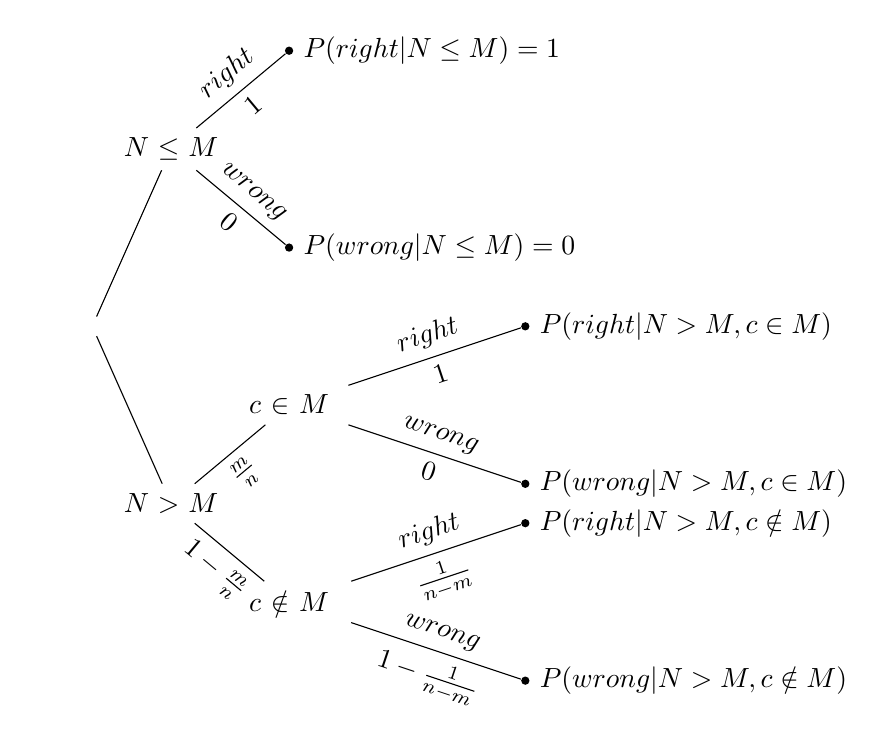
\begin{tikzpicture}[grow=right, sloped]
\node[bag] {}
    child {
        node[bag] {$N > M$}      
            child {
                node[bag] {$c \notin M$}
                    child {
                        node[end, label=right: {$P(wrong | N > M, c \notin M)$}] {}
                        edge from parent
                        node[above] {$wrong$}
                        node[below] {$1 - \frac{1}{n - m}$}
                    }
                    child {
                        node[end, label=right: {$P(right | N > M, c \notin M)$}] {}
                        edge from parent
                        node[above] {$right$}
                        node[below] {$\frac{1}{n - m}$}
                    }
                    edge from parent
                    node[above] {}
                    node[below] {$1 - \frac{m}{n}$}
            }
            child {
                node[bag] {$c \in M$}
                    child {
                        node[end, label=right: {$P(wrong | N > M, c \in M)$}] {}
                        edge from parent
                        node[above] {$wrong$}
                        node[below] {$0$}
                    }
                    child {
                        node[end, label=right: {$P(right | N > M, c \in M)$}] {}
                        edge from parent
                        node[above] {$right$}
                        node[below] {$1$}
                    }
                    edge from parent
                    node[above] {}
                    node[below] {$\frac{m}{n}$}
            }
            edge from parent 
            node[above] {}
            node[below] {}
    }
    child {
        node[bag] {$N \leq M$}        
        child {
            node[end, label=right: {$P(wrong | N \leq M) = 0$}] {}
            edge from parent
            node[above] {$wrong$}
            node[below] {$0$}
        }
        child {
            node[end, label=right: {$P(right | N \leq M) = 1$}] {}
            edge from parent
            node[above] {$right$}
            node[below] {$1$}
        }
        edge from parent         
        node[above] {}
        node[below] {}
    };
\end{tikzpicture}

  \caption{Probability tree}
  \label{tree}
\end{figure}

To get the total probabilities for \textit{right} and \textit{wrong} choices, we 
can sum up the paths.

Note that we ignore the upper half of the tree in summing the paths up, since we 
can not derive probabilities for the first branching. We just add those cases 
individually to our function.

We get the following results:
\begin{align*}
&&P(right | N \leq M) &= 1 \\
&&P(wrong | N \leq M) &= 0 \\
&&P(right | N > M, c \in M) &= \frac{m}{n} \\
&&P(wrong | N > M, c \in M) &= 0 \\
&&P(right | N > M, c \notin M) &= \left(1 - \frac{m}{n}\right) \frac{1}{n-m} \\
&&P(wrong | N > M, c \notin M) &= \left(1 - \frac{m}{n}\right) \left(1 - \frac{1}{n-m}\right)
\end{align*}

We can now pick $P(right | N > M, c \in M)$ and $P(right | N > M, c \notin M)$ to 
calculate the marginal probability $P(right | N > M) = P(right | N > M, c \in M) + P(right | N > M, c \notin M)$.

\begin{align*}
P(right | N > M) &= \frac{m}{n} + (1 - \frac{m}{n}) \frac{1}{n - m} = \frac{m + 1}{n}
\end{align*}

Finally we can define $P_{right}(N, M)$ with $P(right | N \leq M)$ and $P(right | N > M)$:

\begin{align*}
P_{right}(N, M) = 
\begin{cases} 
1             & \mbox{if } N \leq M \\ 
\frac{|M|+1}{|N|} & \mbox{if } N > M
\end{cases}
\end{align*}
